\chapter{Introduction}
\label{ch:Introduction}

\section{Background}
\label{sec:Background}

\subsection{Coastal geomorphology}
\label{subsec:Coastal geomorphology}

Coastal geomorphologies in Lake Michigan are diverse and include shorelines, beaches, bluffs, dunes, and other landforms (Jackson et al., 2013). Two of the most common landforms among them are shoreline and bluff, which are shown in Figure \ref{fig:fig1.1}a. Shoreline is the natural boundary of water body and land , excluding areas modified by human structures such as revetments and ripraps. Natural shorelines are the mostly commonly found along the coast of Lake Michigan, comprising over 80 percent of the total coastline (see Figure\ref{fig:fig1.1}b), with the exception of certain urbanized areas such as Chicago and Milwaukee. The second common coastal feature is glacial till bluff, a vertical landform which is formed by glacial movement (Mickelson et al., 1977, 2004). Bluffs typically rise behind the shoreline and beach, with heights ranging from one to forty meters (Mickelson et al., 2004). In Lake Michigan, bluffs are primarily distributed along the western and eastern coasts, as shown in Figure \ref{fig:fig1.1}c, accounting for approximately 40 percent of the total lake coastline. Both shorelines and bluffs are not only common but also significant, as they are located in or near populated and developed areas such as Chicago and Milwaukee. These areas affect the lives of over 10 million people and protect properties valued at more than 1,000 billion dollars, with an estimated cost of $ \$10,000$ per linear foot of lakefront (Folger et al., 1996). Overall, coastal geomorphologies, especially coastal bluff and shoreline, are both prevalent and important in Lake Michigan coastal environments, necessitating comprehensive and detailed studies.
\begin{figure}[htbp]
  \centering
  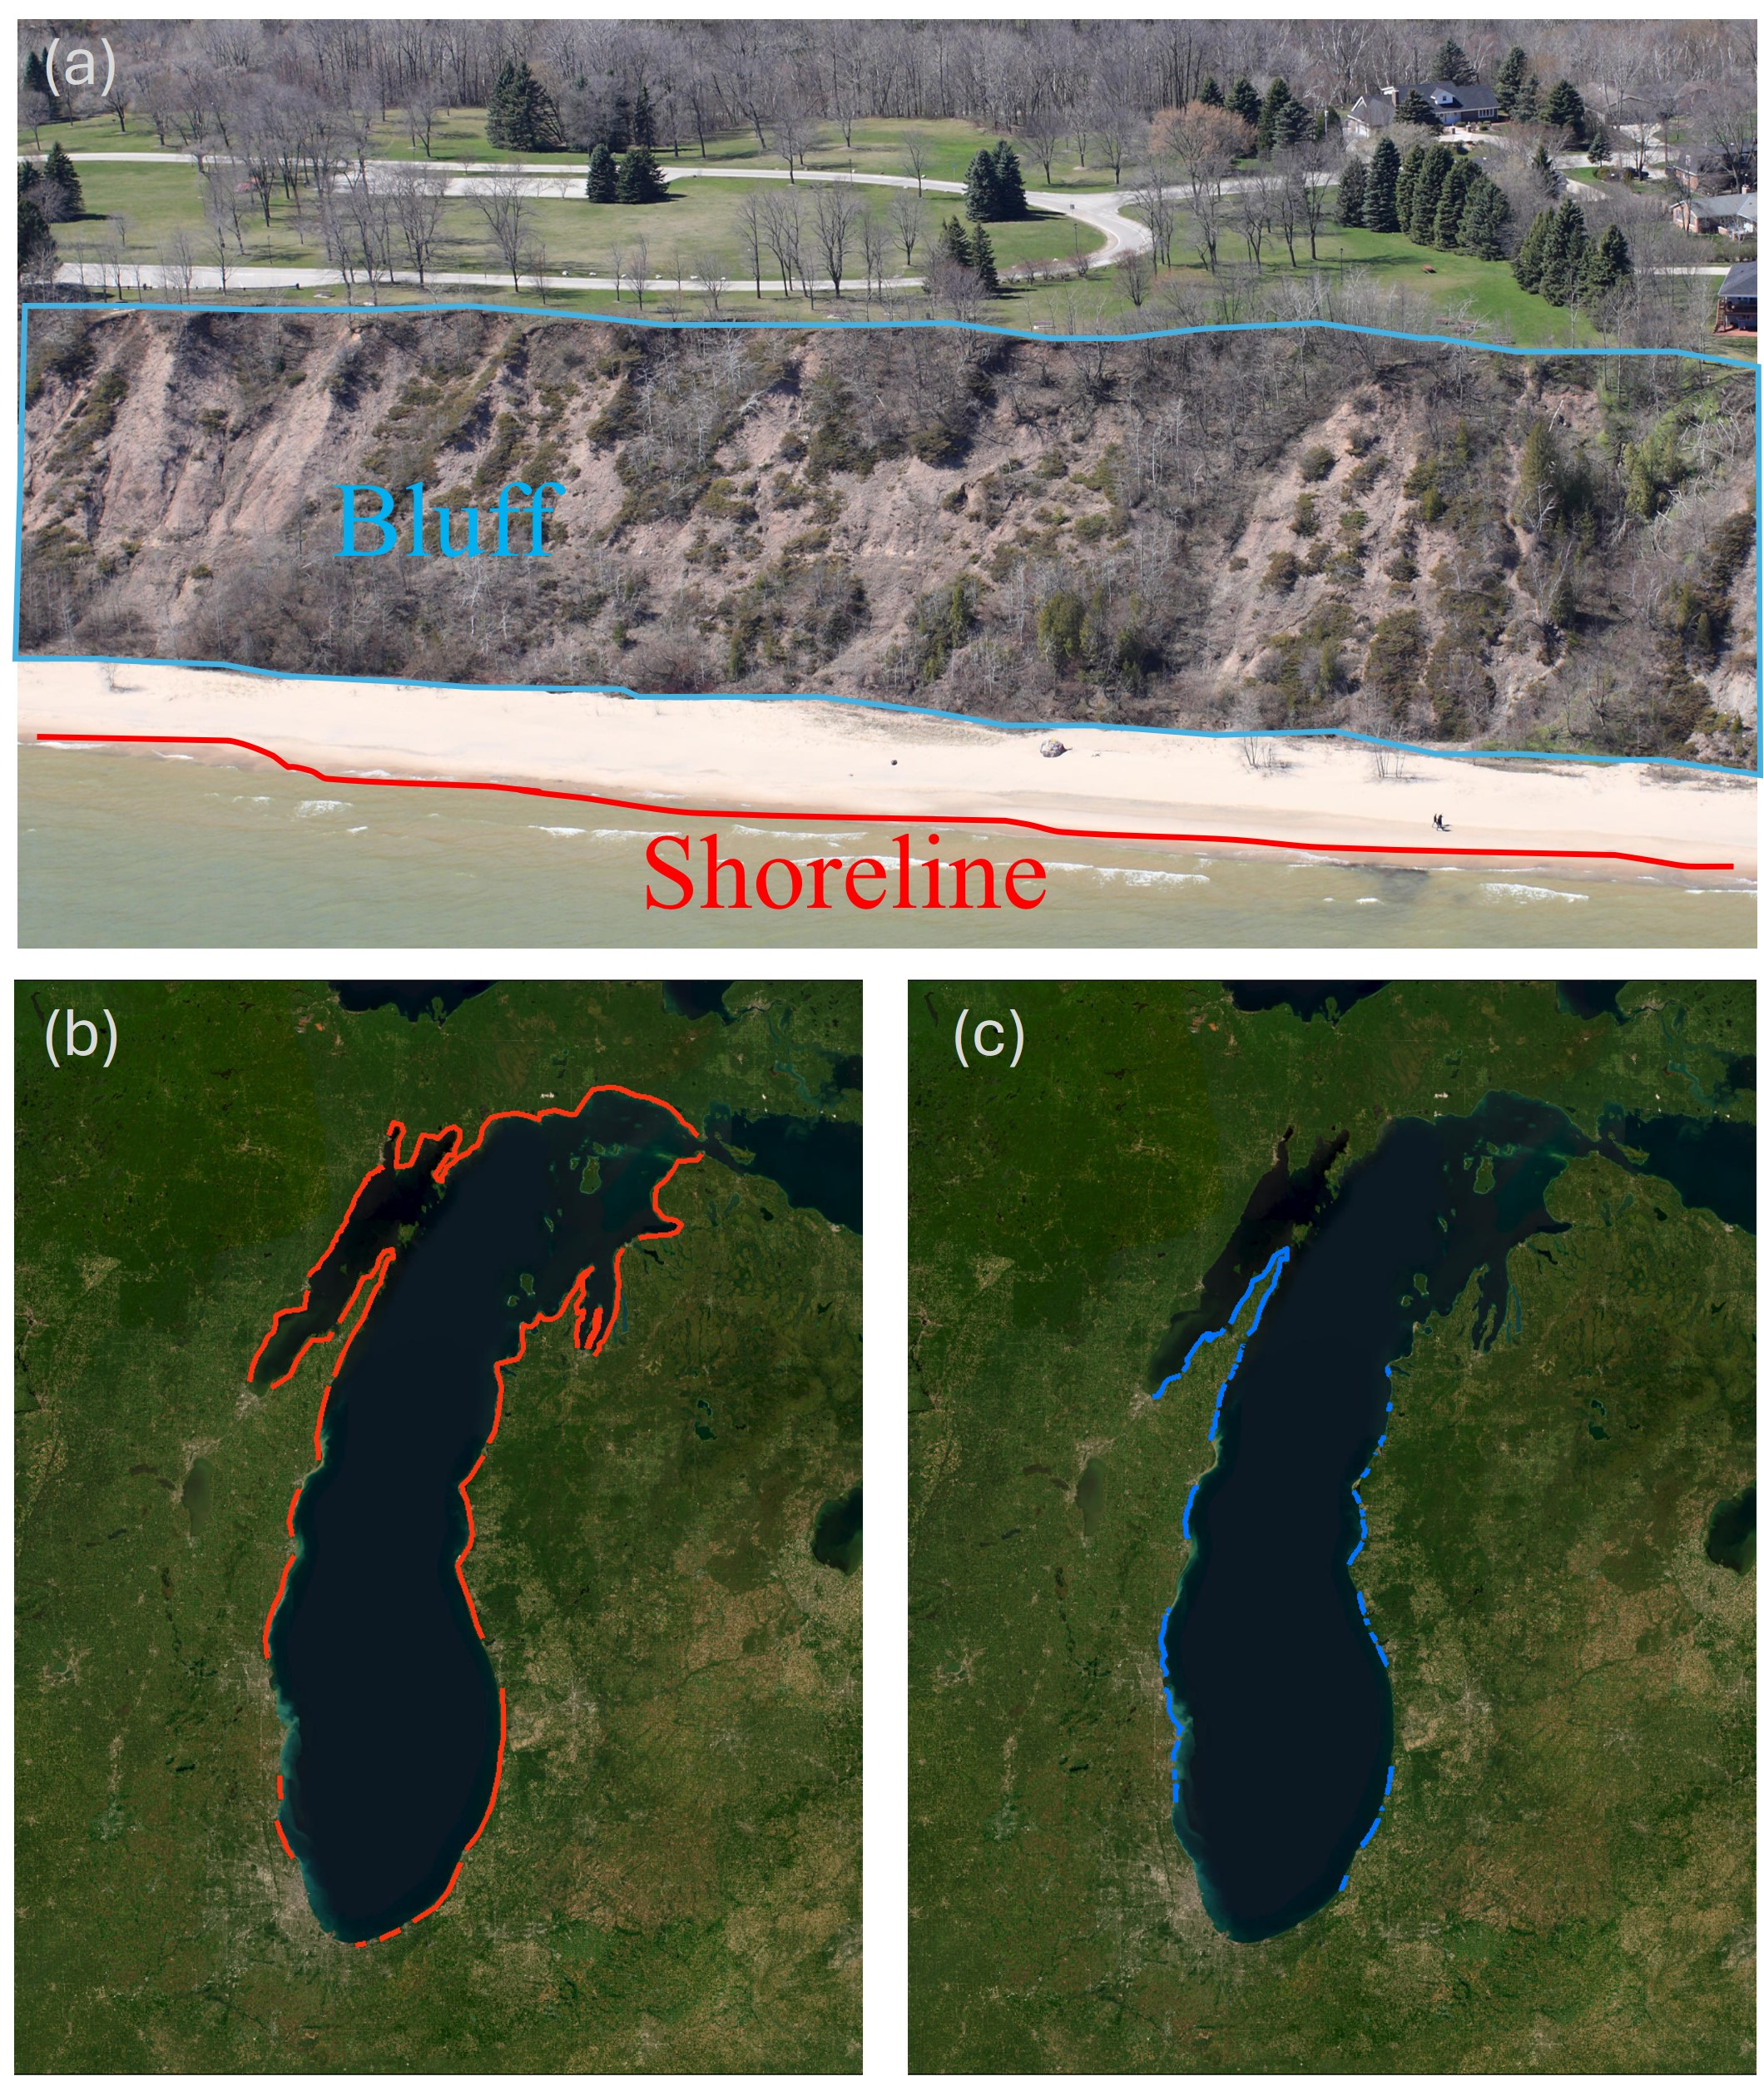
\includegraphics[width=0.8\textwidth]{chapter1/resources/figure1-1.jpg}
  \caption{The common coastal geomorphologies in Lake Michigan. (a) oblique photos of bluff and shoreline (bluff and shoreline), (b) natural shoreline map and (c) bluff map (tall bluffs over 10 meter) in Lake Michigan.}
  \label{fig:fig1.1}
\end{figure}


Coastal geomorphic change (CGC), also known as coastal accretion and erosion, are the evolution and transformation of coastal geomorphology over time (Biswas et al., 2023). CGC is important in the coastal environment because it can cause various coastal hazards. Two of the most common coastal hazards caused by CGC are bluff failure and shoreline retreat (see Figure \ref{fig:fig1.2}), both of which are critically important in coastal environments due to their significant impacts on human infrastructure and ecosystems. Bluff erosion at both the crest and toe of bluff could undermine the stability of bluff structures, potentially leading to a bluff failure. Bluff failure, including collapses, landslides, and slumps, as depicted in Figure \ref{fig:fig1.2}a, is particularly destructive, as it can damage properties and infrastructures built at the top or base of the bluff, leading to economic losses and even casualty (Deitz et al., 2024).  For instance, between 2019 and 2022, there were three reported news (Mitchell, 2019; Fromson, 2020; Koran, 2022) of homes collapsing due to unstable coastal bluffs in Lake Michigan. Another common issue is shoreline retreat, which is well-known for its adverse effects on coastal and nearshore ecosystems, as well as biodiversity. For instance, dune ecosystems, which provide dynamic habitats for species such as beach grass, sand verbena, and plovers, can be severely degraded by shoreline retreat (Van der Biest et al., 2017). Recently, CGC has become an urgent issue, as accelerated erosion along coastal bluffs and shorelines has been observed, reaching its highest rate in the past 30 years.  Facing threats from these two issues, numerous efforts have been made. For example, in southeastern Wisconsin, over $2.89$ billion was spent to construct, repair and maintain the structures to protect the local properties and infrastructure (WEM, 2016). Despite these considerable expenditures to mitigate the risks of CGC, there remains an additional critical step: coastal geomorphology mappings on multiple temporal and spatial scales. Multi-scale coastal mapping can provide insights into the evolution of coastal geomorphology across varying temporal and spatial scales, offering valuable guidance and perspectives for effective prediction and prevention for coastal hazards (Mongus, 2014; Papakonstantinou et al., 2016). In Lake Michigan, although numerous projects and studies have been made for characterization of coastal geomorphic change, most have been limited to small regions or short time periods, leaving multi-spatial and multi-temporal CGC insufficiently explored. Given the lack of a clear characterization of CGC, it would be valuable to conduct an extensive mapping and analysis across the coastal region of southwestern Lake Michigan to address gaps in understanding CGC over multi-spatial and multi-temporal scales.

\begin{figure}[htbp]
  \centering
  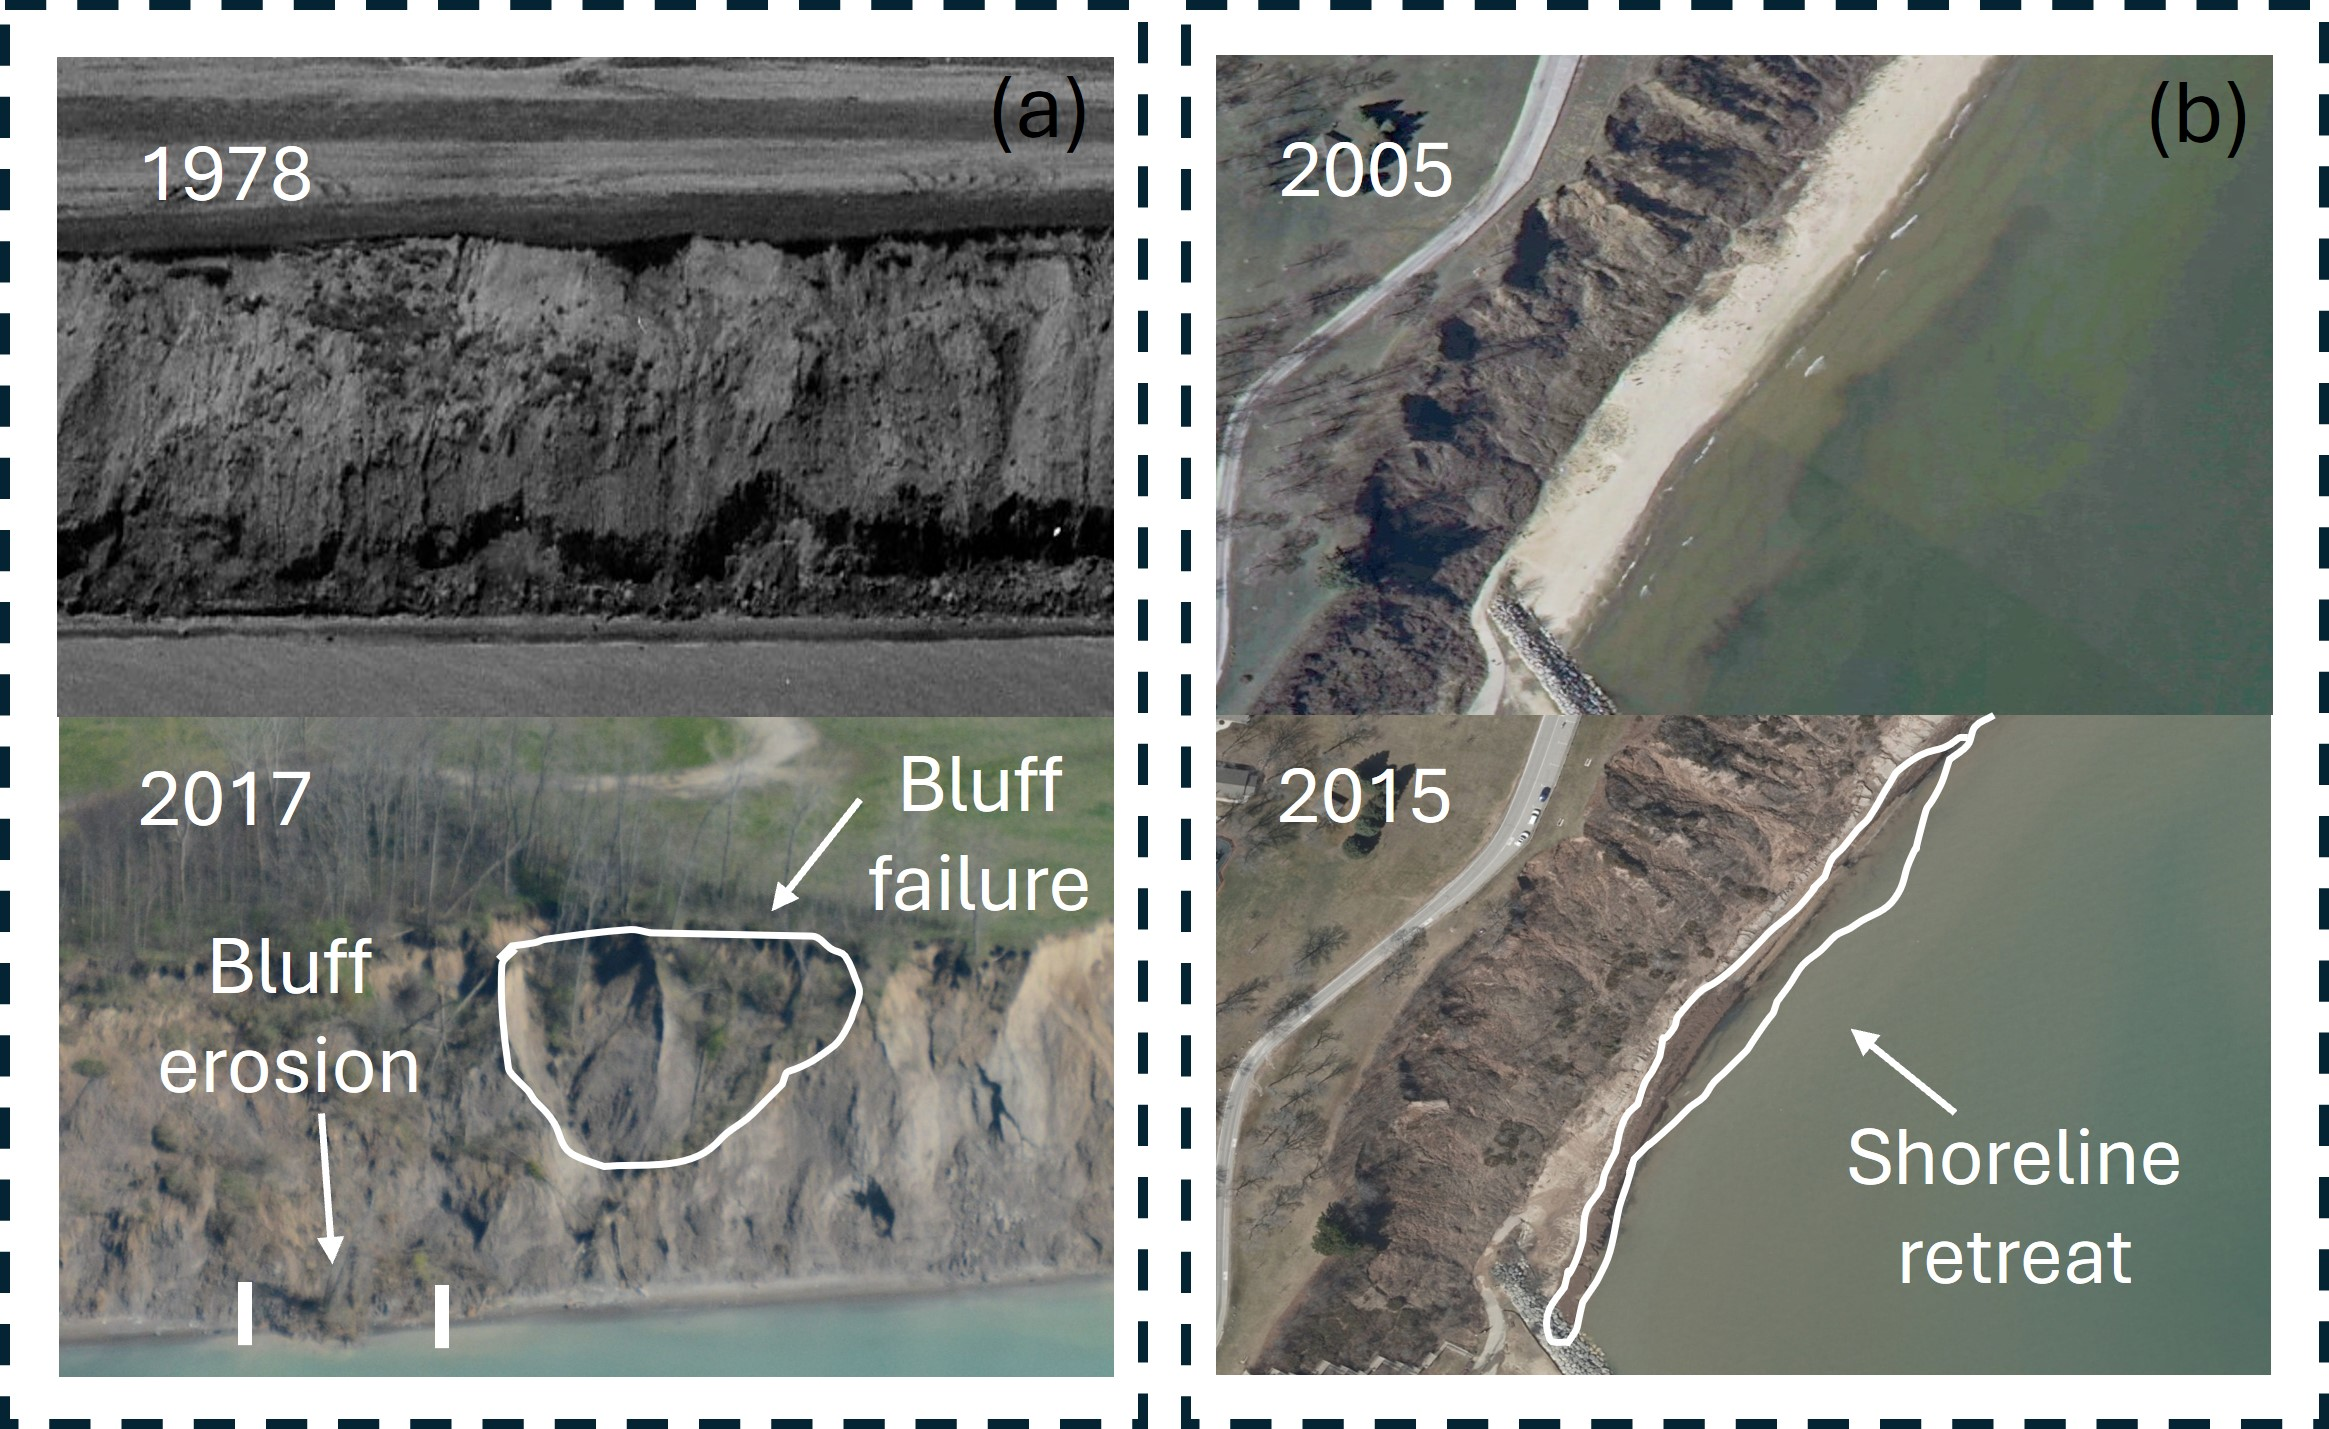
\includegraphics[width=0.8\textwidth]{chapter1/resources/figure1-2.jpg}
  \caption{images that show two typical hazards caused by CGC: (a) bluff failure, (b) shoreline retreat.}
  \label{fig:fig1.2}
\end{figure}


\subsection{Climatology of water level and wind wave}
\label{subsec:Climatology of water level and wind wave}

There are two important hydrodynamic processes that significantly affect coastal geomorphology: water level and wave. The climatology of water level, which refers to the study of the elevation fluctuation of lake or sea surface, is the most well-studied topic in the coastal region. The climatology of water level is important as it implies the stability of coastline, health of coastal habitat, and safety of ship navigation (Posey, 2012) etc. To better understand the climatology of hydrodynamic process, numerous efforts have been made. For example, in the Great Lakes, the records of water levels were initially documented since the 1820s and have been systematically monitored across the lakes since the 1920s by NOAA. In Lake Michigan, NOAA has deployed 10 water level gauges since the 1970s to monitor monthly lake level fluctuations with verification, as shown in Figure \ref{fig:fig1.3}. These long-term data have allowed for a comprehensive understanding of lake level climatology, including inter-annual trend (Hanrahan et al., 2014; Chen et al., 2022), seasonal cycles (Argyilan and Forman, 2003; Quinn, 2002), and daily events (Trebitz, 2006). Furthermore, the mechanisms driving lake level fluctuations have been widely explored, including factors such as precipitation (Rodionov, 1994; Hanrahan et al., 2014), runoff and evaporation (Gronewold et al., 2016; Cheng et al., 2021), ice cover (Farhadzadeh, 2017), and atmospheric teleconnections (Ghanbari and Bravo, 2008).

\begin{figure}[htbp]
  \centering
  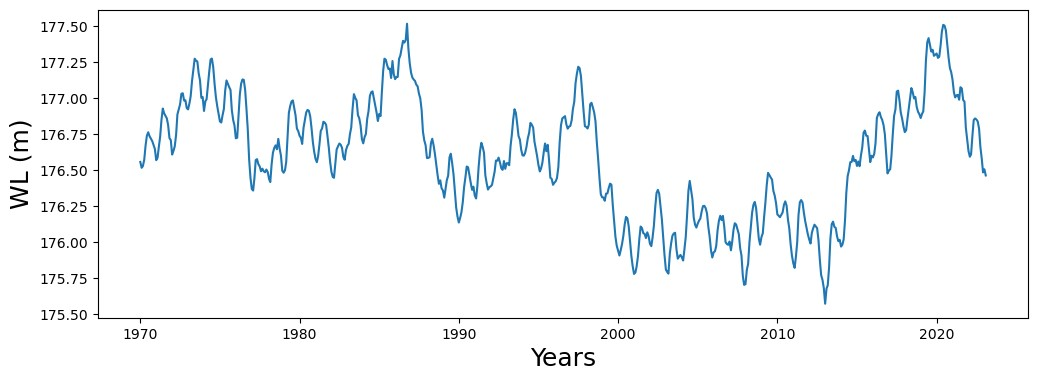
\includegraphics[width=0.8\textwidth]{chapter1/resources/figure1-3.jpg}
  \caption{Monthly water level fluctuation in Lake Michigan from NOAA tide\&current.}
  \label{fig:fig1.3}
\end{figure}

Wind wave, a periodic circular motion of fluid driven by wind force, is another important nearshore process, as it is closely related to water level fluctuation (Meadows et al., 1997; Huang et al., 2021), coastal structure constructions (Karambas, 2015), and coastal energy generation (Ching-Piao et al., 2012). Similar to water level, wave climatology is key to understanding the hydrodynamic property of wave processes. Nevertheless, compared to the climatology of water level, which primarily focuses on magnitude of lake elevation, the wind wave climate involves a broader range of wave characteristics such as wave directionality and wave spectrum, due to the more complex nature of wave processes. For example, waves can be bent perpendicular to the contours of the bathymetry as wave propagates in different water depths, which is known as the wave refraction. The wave refraction often results in uni-directional wave climate on the coast where all waves are bent perpendicular to the shoreline (see Figure \ref{fig:fig1.4}a). Conversely, when waves encounter obstacles like groins or breakwaters, they can bend into a bi-directional pattern, traveling in opposite or oblique directions due to wave diffraction (see Figure \ref{fig:fig1.4}b). Both uni-directional and bi-directional wave climates are commonly observed in Lake Michigan (see Figure \ref{fig:fig1.4}c), and are important for navigation safety (Zimmermann et al., 2012), wave energy farm construction (López-Ruiz et al., 2016; Bertram et al., 2020), and beach rotation (Wiggins et al., 2019a; Wiggins et al., 2019b). Another important wave process is wave systems. Wind waves can be classified into two wave systems: wind-sea and swell, which represent different wave states. Wind-sea refers to waves generated by local winds, typically characterized by longer wave periods and less developed waveforms. In contrast, swell refers to waves that have grown and propagated beyond the influence of the wind that originally generated them. Swells can travel long distances with minimal energy loss and are distinguished by their shorter wave period (Ardhuin et al., 2009). In wave climatology, windsea and swell are regarded as two components of the spectral wave climate, and spectral wave climate is important for wind wave data reduction, model validation, and wave event tracing (Portilla-Yandún et al., 2015). In summary, wind wave climate involves more complex wave characteristics such as wave height, wave energy, wave direction, wave spectrum. In Great Lakes, most studies of wave climates have focused on the annual or monthly trend of wave height (e.g. Olsen, 2019; Huang et al., 2021) or wave energy (e.g. Meadows et al., 1997). To date, the directional and spectral wave climate in the Great Lakes has not yet been revealed. Hence, further exploring to understand the directional spectral wave climate in Lake Michigan may shed light on complex hydrodynamic processes.

\begin{figure}[htbp]
  \centering
  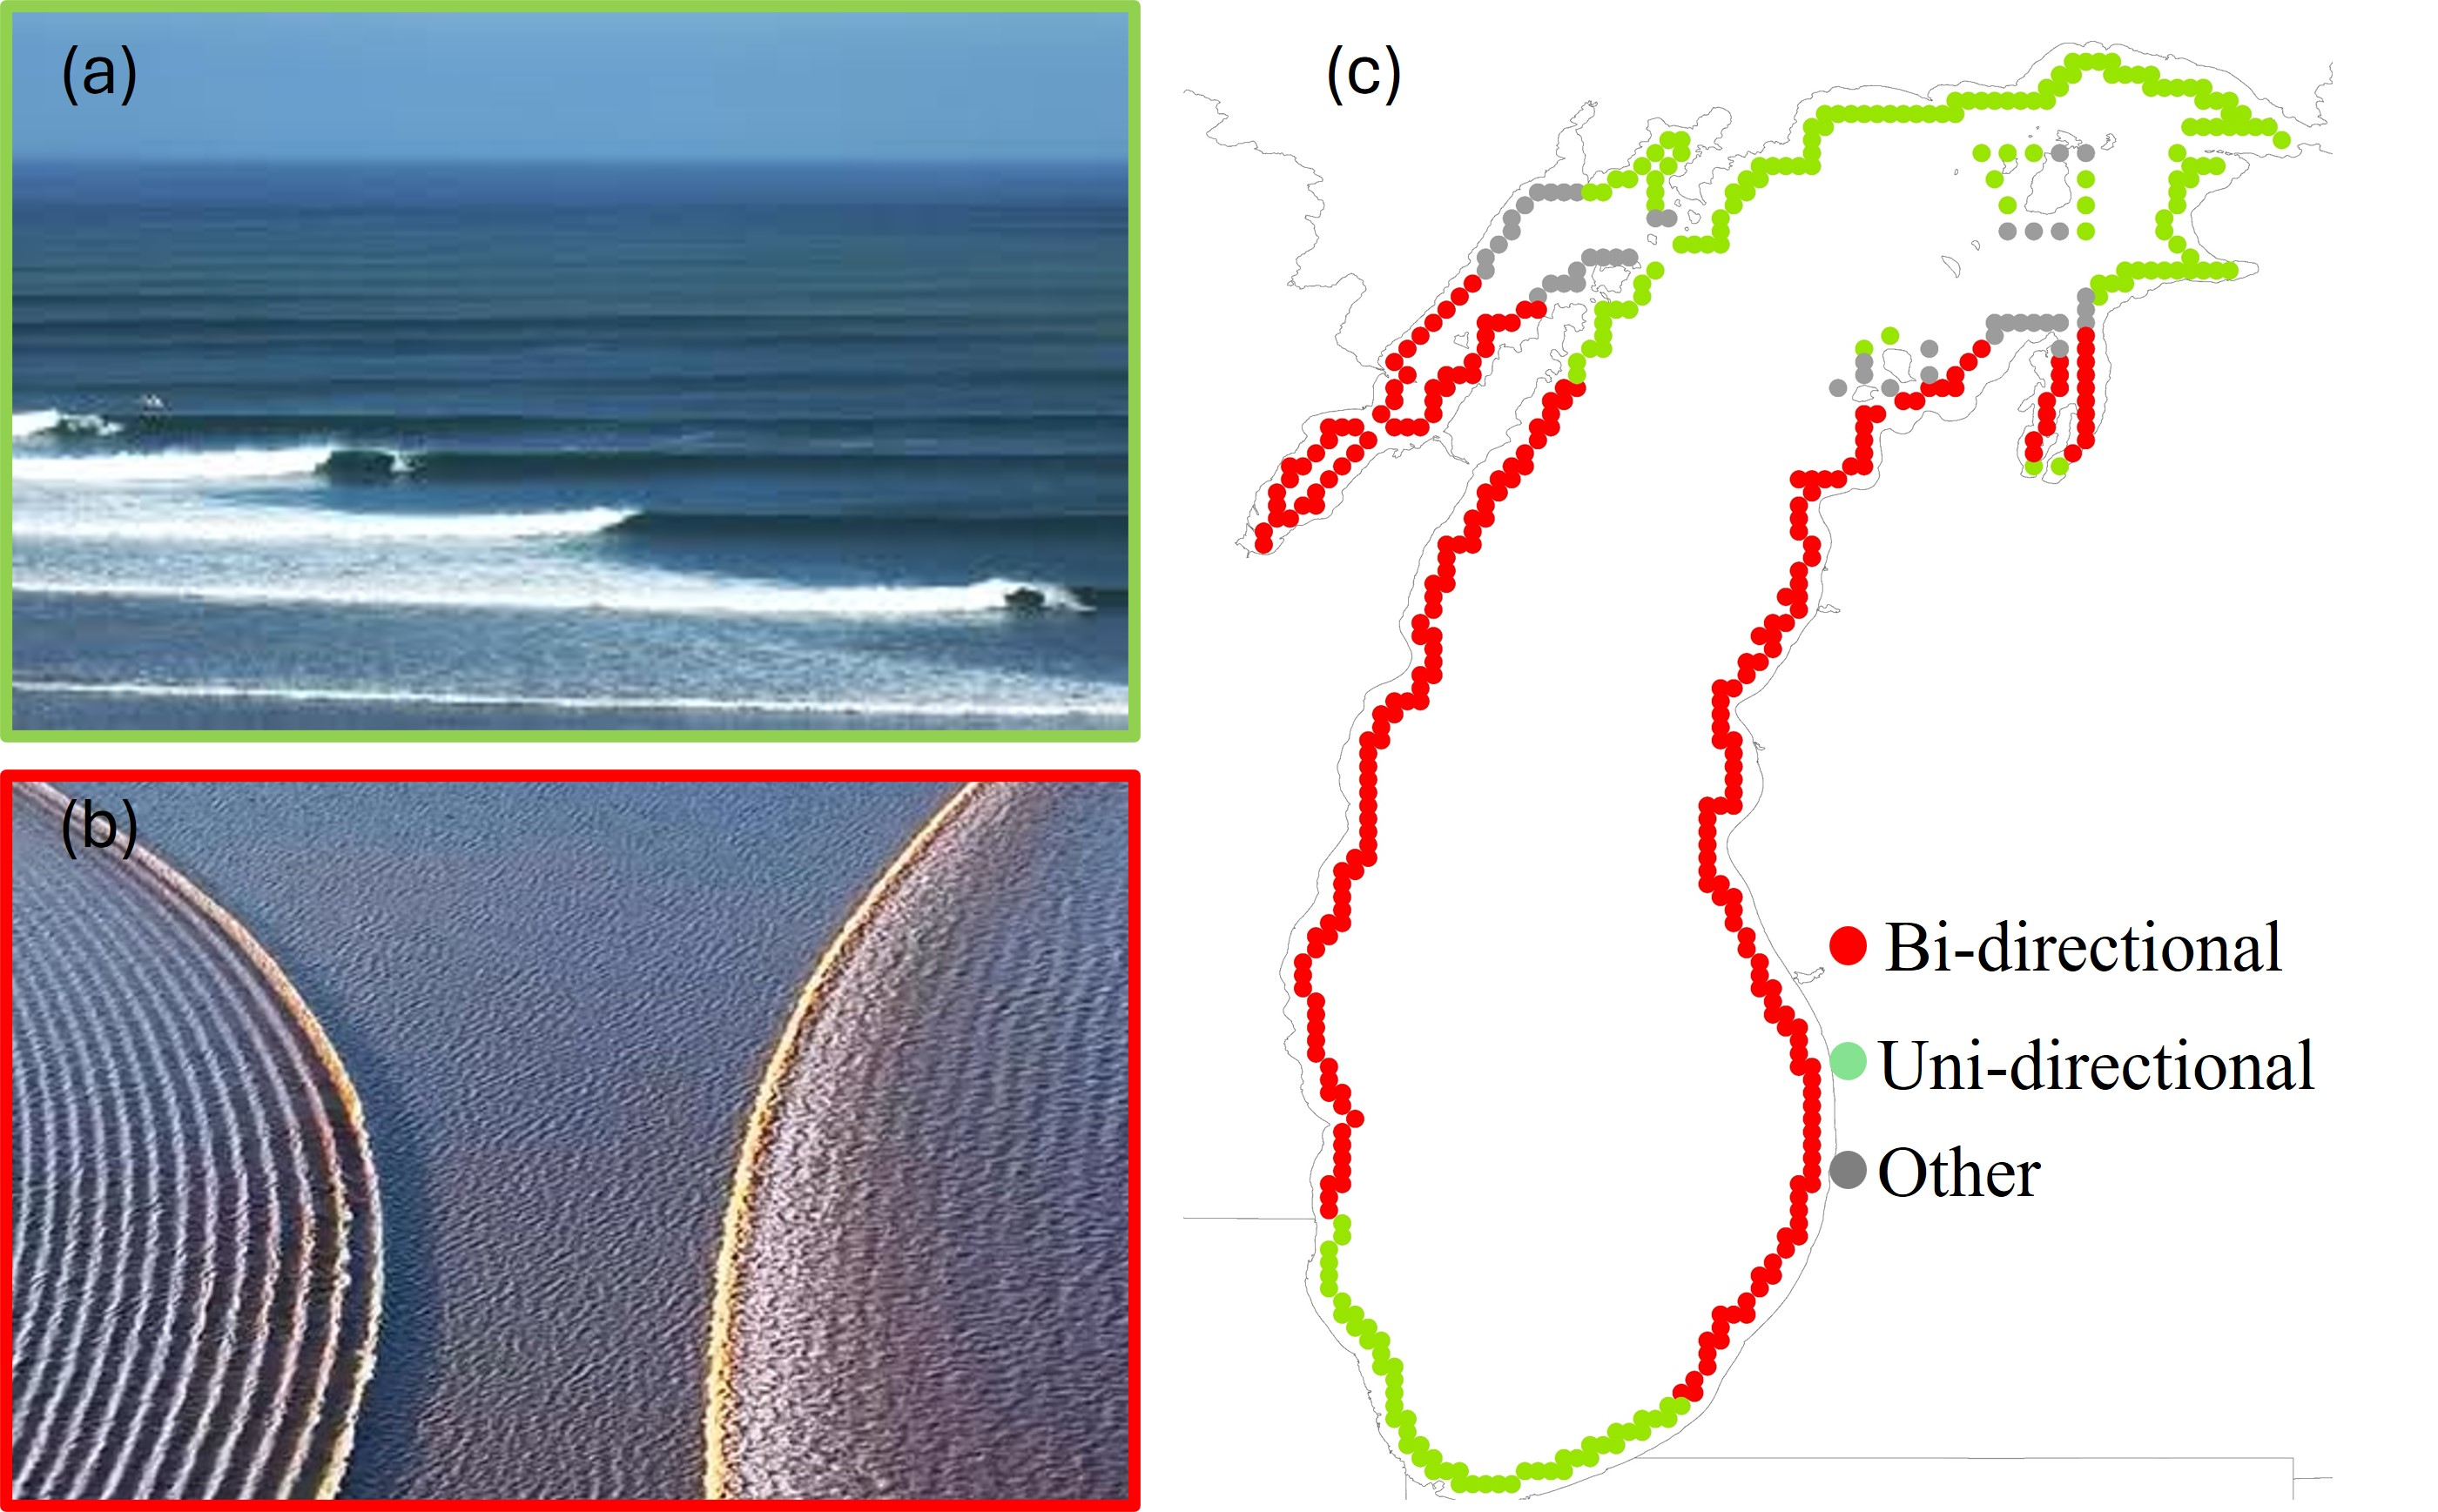
\includegraphics[width=0.8\textwidth]{chapter1/resources/figure1-4.jpg}
  \caption{The photos of directional wave climate: (a) uni-directional and (b) bi-directional, associated with (c)the maps of the directional wave climate in Lake Michigan.}
  \label{fig:fig1.4}
\end{figure}

\subsection{Relationship between coastal geomorphology and wave climate}
\label{Relationship between coastal geomorphology and wave climate}

It is well-known that water level could significantly influence the coastal environment in Great Lakes, including wetland habitat (Hohman et al., 2021; Anderson et al., 2023), sandy dunes, bluff (Volpano et al., 2020) and beach.  Nevertheless, wave climates, especially wave height, directionality, and wave systems, are sometime ignored for its huge impact on coastal geomorphologies including shoreline and bluff. For example, wave height determines the wave energy flux, which is regarded as an important indicator as coastal bluff erosion and shoreline recession. Wave height can be further amplified through wave shoaling effect (Figure \ref{fig:fig1.5}a) and refraction effect (Figure \ref{fig:fig1.5}b), leading to a steeper lakebed and bluff face, which causes accelerated erosion in the shoreline and failure in bluff (Booth, 1994). Moreover, the wave-driven nearshore sediment transport can also lead to the redistribution of nearshore sediment budgets, which is essential to shoreline erosion. Cumulative wave impact height, which is an index derived from the nearshore wave height and water level, was also found to be a control of the coastal erosion (Ruggiero et al., 2001; Swenson et al., 2006). Wave directionality and wave systems are also found to be highly related to coastal geomorphology. For example, numerous studies found that bidirectional wave climate, a special wave directionality with two opposite wave directions, can cause coastal beach rotation, which is a common coastal process occurred at many semi-sheltered and embayed shorelines (Klein et al., 2002; Wiggins et al., 2019b; Loureiro and Ferreira, 2020). However, despite of the fact that wave climate could impact coastal geomorphic changes, the relationship between coastal geomorphic change and wind wave climate, particularly directionality and wave systems, is still under-studied yet. 

\begin{figure}[htbp]
  \centering
  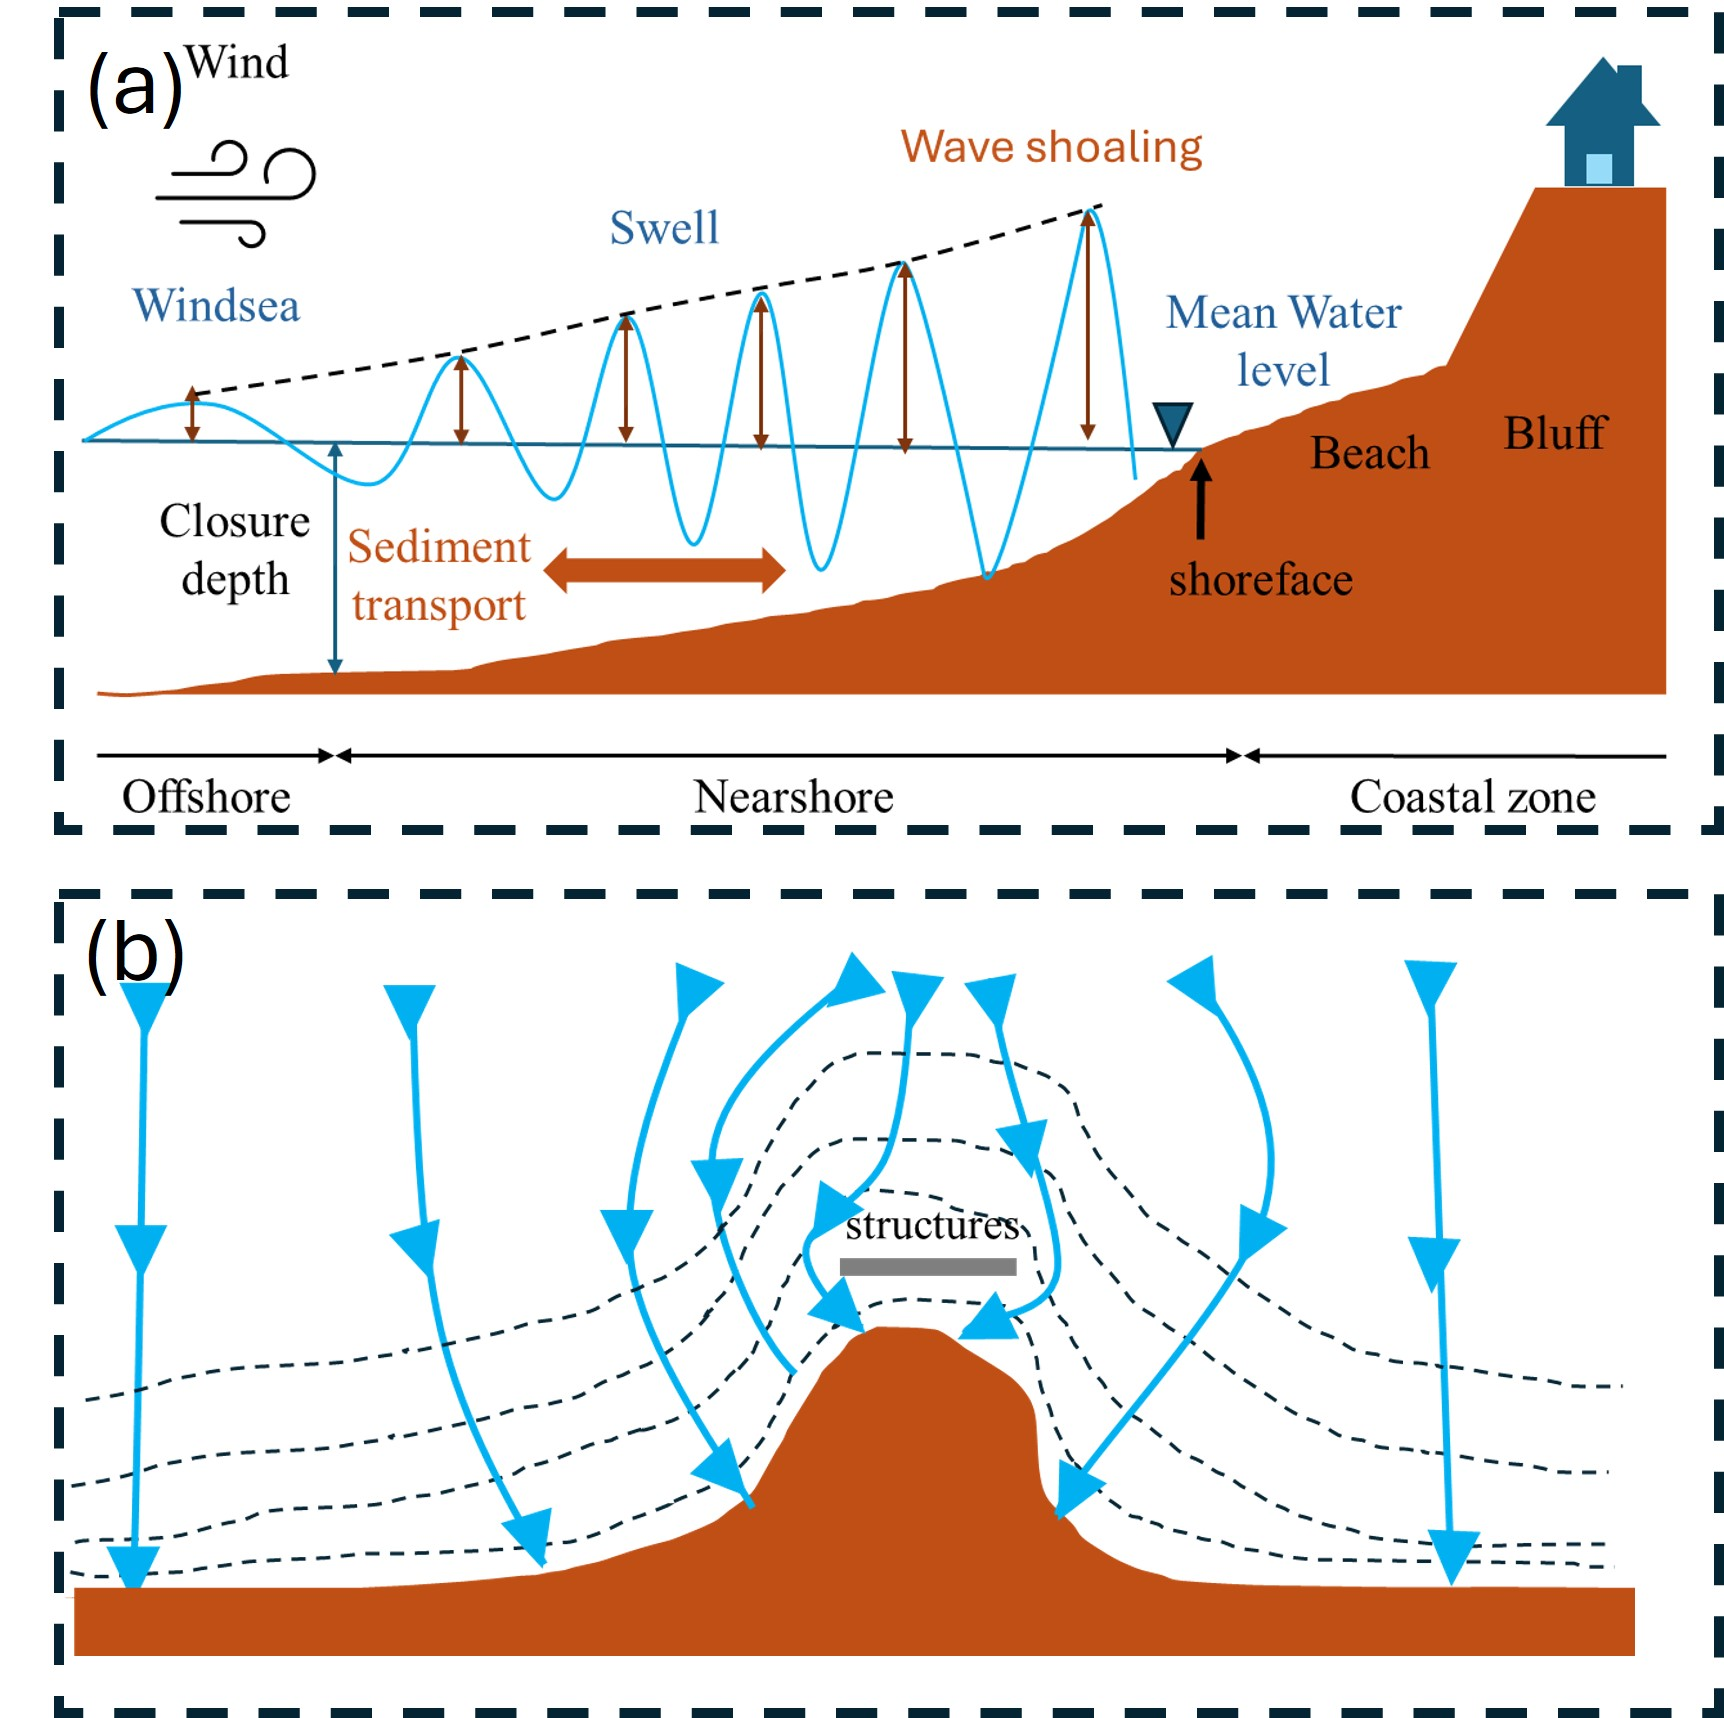
\includegraphics[width=0.8\textwidth]{chapter1/resources/figure1-5.jpg}
  \caption{wave climates in the coastal environment: (a) wind wave including windsea and swell under shoaling effect, (b) refraction and diffraction.}
  \label{fig:fig1.5}
\end{figure}


\section{Research questions and objectives}

To date, the importance of coastal geomorphic changes and wind wave climate has been widely recognized in the world. However, in Lake Michigan, several knowledge gaps persist, limiting our understanding of these critical processes, which leads to the formulation of the following research questions:

\begin{enumerate}
    \item Coastal geomorphology: What are the multiple scales of coastal geomorphic changes on Lake Michigan?
    \item Wind wave climate: What are the characteristics of wind wave climate, especially directionality and wave systems in Lake Michigan?
    \item Relationships: How to indicate the CGC with the assistant of directional spectral wave climate?
\end{enumerate}

In response to these three unanswered questions, the proposed research objectives are: (1) to characterize coastal geomorphological changes and wind wave climate in Lake Michigan, and (2) to investigate the relationship between them. This research is structured into four chapters, each addressing critical gaps to answer the overarching research questions regarding coastal geomorphological changes and wind wave climates. The specific research question, objective, and contribution for each chapter are summarized in the following table:

\renewcommand{\arraystretch}{1.4}

\begin{longtable}{|>{\raggedright\arraybackslash}p{2.4cm}|p{12cm}|}
\caption{Chapter Overview} \\
\hline
\multicolumn{2}{|c|}{\textbf{Chapter 2}} \\
\hline
\textbf{Topic} & \textit{Coastal geomorphological changes on southwestern Lake Michigan: Perspective from multi-scale} \\
\textbf{Question} & What are the coastal geomorphological changes on multi-scale in the coastline of southwestern Lake Michigan? \\
\textbf{Objective} & To characterize coastal geomorphological changes on different temporal and spatial scales. \\
\textbf{Contribution} & Provide an insight of bluff and shoreline change over both long-term and short-term periods, utilizing three distinct spatial scales. \\
\hline
\multicolumn{2}{|c|}{\textbf{Chapter 3}} \\
\hline
\textbf{Topic} & \textit{Wave climate on the southeastern Wisconsin coast of Lake Michigan: Perspective from wave directionality} \\
\textbf{Question} & Does wave directionality help identify the trend of wave climate? \\
\textbf{Objective} & To characterize the directional wave climate in the nearshore of southeastern Lake Michigan. \\
\textbf{Contribution} & Provide an approach to define the wave directionality and explore the implication of wave directionality. \\
\hline
\multicolumn{2}{|c|}{\textbf{Chapter 4}} \\
\hline
\textbf{Topic} & \textit{Wave climate on the southeastern Wisconsin coast of Lake Michigan: Perspective from wave systems} \\
\textbf{Question} & Does wave spectrum help identify the trend of wave climate? \\
\textbf{Objective} & To analyze the effect of swells and wind–sea waves at the nearshore of Lake Michigan. \\
\textbf{Contribution} & Illustrate the trend of wave climate by swell–wind–sea separation and by probability distribution in spectral occurrence map. \\
\hline
\multicolumn{2}{|c|}{\textbf{Chapter 5}} \\
\hline
\textbf{Topic} & \textit{Assessing coastal vulnerability using directional spectral wave climate: Coastal Vulnerability Index} \\
\textbf{Question} & How does the directional spectral wave climate impact the coastal vulnerability? \\
\textbf{Objective} & Develop an index to access the coastal vulnerability that is applicable to the directional spectral wave climate in Lake Michigan. \\
\textbf{Contribution} & Provide an insight in coastal vulnerability in Lake Michigan coastline. \\
\hline
\end{longtable}


In summary, this study aims to advance the understanding of coastal geomorphology and wind wave climate, as well as the intricate relationship between them.
% Your chapter content goes here...
